\documentclass[11pt]{article}
\usepackage[margin=1in]{geometry}
\usepackage{amsmath, amssymb, amsthm}
\usepackage{physics}
\usepackage{bm}
\usepackage{hyperref}
\usepackage{graphicx}
\usepackage{enumitem}
\usepackage{siunitx}

\usepackage{mathtools}
\usepackage{braket}
\usepackage{quantikz}
\usepackage{tikz}
\usepackage{tikz-3dplot}
\usetikzlibrary{arrows.meta,calc}
\usepackage{MnSymbol,wasysym}

\title{CSCI-739 Quantum Machine Learning\\[2pt]
\large Homework 1}
\date{} % <-- leaving empty removes today's date
\setlist[itemize]{left=1.25em}
\setlist[enumerate]{left=1.25em}
\newcommand{\pts}[1]{\hfill{\small\bfseries(#1 pts)}}
\newenvironment{summary}{\vspace{2pt}\noindent\textbf{Summary.}~}{\par\vspace{6pt}}

\newcounter{problem}
\newcommand{\problem}[2]{% #1 = title, #2 = points
  \refstepcounter{problem}
  \vspace{10pt}\noindent\textbf{Problem \theproblem.~#1} \pts{#2}\par
}

\newcounter{bonus}
\newcommand{\bonus}[2]{% #1 = title, #2 = points
  \refstepcounter{bonus}
  \vspace{10pt}\noindent\textbf{Bonus \Alph{bonus}.~#1} \pts{#2}\par
}

\begin{document}
\maketitle

\begin{center}
\textit{You got this team. My homeworks are meant to to help you get on the path to become a quantum nerd like me. Well, that is if you would like to be one someday \smiley{}. Remember if Ryan Vogt can do quantum computing, that means anyone can! }
\end{center}

\vspace{1em}

\noindent
*uhum inspirational speech*

Quantum computing is not just another incremental advance in technology—it is the beginning of a paradigm shift in how we process information, solve problems, and imagine the future of computation. In the coming years, quantum computers will transform machine learning, offering the possibility of speedups and entirely new frameworks for representing and reasoning about data. Quantum Machine Learning (QML) sits at this frontier: a discipline that blends the strange power of quantum mechanics with the most transformative computational tool of our time, machine learning. 

By working through this homework, you are starting to develop the fundamental skills—linear algebra, quantum gates, circuits, and measurement—that form the foundation of this field. Each problem is designed to build your ability to reason like a quantum scientist, and to prepare you to unlock the potential of QML. What begins here with single qubits and simple circuits will eventually connect to the exponential potential of quantum-enhanced learning systems. This is the path forward, and you are now taking the first steps.

Go research, use the lecture notes, videos, and the internet. The world is your quantum oyster team \smiley{}.

\vspace{1em}

% ---------------- Homework Summary ----------------
\section*{Homework Summary}
This homework contains five standard problems (20 points each) and two bonus problems (25 points each). Together they guide you through the basics of quantum computing, which are the building blocks to facilitate QML.

\begin{enumerate}
  \item \textbf{Qubit Basics:} Probabilities, normalization, and measurement with Dirac notation.
  \item \textbf{Two-Qubit Systems and CNOT:} Basis states via tensor products, amplitudes, CNOT action, and flipped-control CNOT unitarity.
  \item \textbf{The Bloch Sphere and Single-Qubit Gates:} Mapping amplitudes to $(\theta,\phi)$, analyzing gate actions, and interference with Hadamards.
  \item \textbf{From Tensor Products to Circuits:} Proving tensor-product properties and building equivalent Qiskit circuits.
  \item \textbf{Ripple-Carry Adder:} Implementing and interpreting a 1-bit ripple-carry adder in Qiskit.
  \item[\textbf{Bonus A.}] \textbf{Time-Dependent Schr\"odinger Equation:} Operator solutions, unitarity, and engineered Hamiltonians for gates.
  \item[\textbf{Bonus B.}] \textbf{Adding 2+2 on a Quantum Computer:} Building a 2-bit ripple-carry adder and verifying results via simulation, and an optional addition is to test it on real hardware.
\end{enumerate}

% ---------------- Problem 1 ----------------
\problem{Qubit Basics}{20}
\begin{summary}
This problem introduces the fundamental concept of a single qubit state and how measurement is related to its amplitudes. You will calculate probabilities using Dirac notation and confirm normalization for a specific example.
\end{summary}

Consider a general single-qubit quantum state:
\[
\ket{\psi} = \alpha \ket{0} + \beta \ket{1}, \quad \text{with } \alpha, \beta \in \mathbb{C}, \ |\alpha|^2 + |\beta|^2 = 1.
\]

\begin{enumerate}[label=(\alph*)]
  \item Write the expression for the probability of measuring the qubit in the state $\ket{0}$ and in the state $\ket{1}$, using inner products (bra-ket notation).
  \item Verify that the sum of the two probabilities is always equal to $1$.
  \item For the specific state 
  \[
  \ket{\psi} = \tfrac{1}{\sqrt{2}}\ket{0} + \tfrac{1}{\sqrt{2}}\ket{1},
  \]
  calculate explicitly the probability of obtaining $\ket{0}$ and of obtaining $\ket{1}$.
\end{enumerate}

% ---------------- Problem 2 ----------------
\problem{Two-Qubit Systems and CNOT}{20}
\begin{summary}
This problem extends your understanding from single qubits to two-qubit systems. You will define the computational basis states using tensor products, analyze how quantum gates act on these states, and explore the structure of the CNOT operation.
\end{summary}

\begin{enumerate}[label=(\alph*)]
  \item Define each of the four basis states $\ket{00}, \ket{01}, \ket{10}, \ket{11}$ explicitly using tensor product notation between single-qubit states, and then write the vector representation of each of the four basis states.
  \item Consider the two-qubit state
  \[
    \ket{\psi} = \sqrt{\tfrac{1}{10}}\ket{00} + \sqrt{\tfrac{4}{10}}\ket{01} + \sqrt{\tfrac{2}{10}}\ket{10} + \sqrt{\tfrac{3}{10}}\ket{11}.
  \]
  Verify normalization and state the probability of each basis outcome. \textit{Note: In this example the amplitudes are real, but in general they are complex, and the probability is the modulus squared of the amplitude.}
  \item Compute the probability of measuring each basis state after applying a CNOT gate with the left qubit as control and the right as target.
  \item Derive the $4\times 4$ unitary matrix of the flipped-control CNOT (right controls, left is target). \textit{Hint:} track where each basis state maps under this assumption, and create a unitary matrix that would map each basis state to the expected operation.
  \item Prove that the matrix in (d) is unitary.
\end{enumerate}

% ---------------- Problem 3 ----------------
\problem{The Bloch Sphere and Single-Qubit Gates}{20}
\begin{summary}
This problem develops your understanding of the Bloch sphere representation of a qubit and how single-qubit gates act on quantum states. You will translate between amplitude form and Bloch sphere parameters, analyze the action of common gates, and explore interference effects through repeated Hadamard operations.
\end{summary}

\begin{enumerate}[label=(\alph*)]
  \item Any single-qubit state can be written as
  \[
    \ket{\psi} = \cos\!\left(\tfrac{\theta}{2}\right)\ket{0} + e^{i\phi}\sin\!\left(\tfrac{\theta}{2}\right)\ket{1}, 
  \]
  where $\theta\in[0,\pi]$, $\phi\in[0,2\pi)$.  
  Derive $\theta$ and $\phi$ in terms of amplitudes $\alpha,\beta$ for $\ket{\psi}=\alpha\ket{0}+\beta\ket{1}$. State $(\theta,\phi)$ for $\ket{0}$ and $\ket{1}$.
  
  \begin{center}
  \tdplotsetmaincoords{70}{110}
  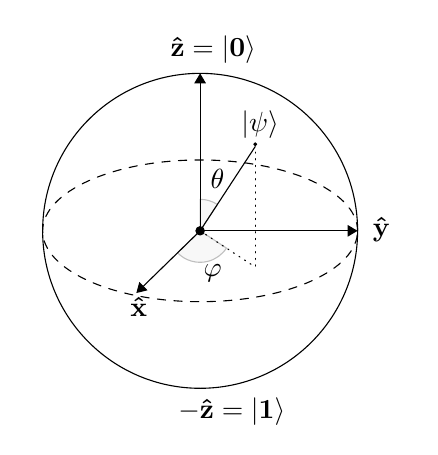
\begin{tikzpicture}[line cap=round, line join=round, >=Triangle]
  \clip(-2.19,-2.49) rectangle (2.66,2.58);
  \draw [shift={(0,0)}, lightgray, fill, fill opacity=0.1] (0,0) -- (56.7:0.4) arc (56.7:90.:0.4) -- cycle;
  \draw [shift={(0,0)}, lightgray, fill, fill opacity=0.1] (0,0) -- (-135.7:0.4) arc (-135.7:-33.2:0.4) -- cycle;
  \draw(0,0) circle (2cm);
  \draw [rotate around={0.:(0.,0.)},dash pattern=on 3pt off 3pt] (0,0) ellipse (2cm and 0.9cm);
  \draw (0,0)-- (0.70,1.07);
  \draw [->] (0,0) -- (0,2);
  \draw [->] (0,0) -- (-0.81,-0.79);
  \draw [->] (0,0) -- (2,0);
  \draw [dotted] (0.7,1)-- (0.7,-0.46);
  \draw [dotted] (0,0)-- (0.7,-0.46);
  \draw (-0.08,-0.3) node[anchor=north west] {$\varphi$};
  \draw (0.01,0.9) node[anchor=north west] {$\theta$};
  \draw (-1.01,-0.72) node[anchor=north west] {$\mathbf {\hat{x}}$};
  \draw (2.07,0.3) node[anchor=north west] {$\mathbf {\hat{y}}$};
  \draw (-0.5,2.6) node[anchor=north west] {$\mathbf {\hat{z}=|0\rangle}$};
  \draw (-0.4,-2) node[anchor=north west] {$-\mathbf {\hat{z}=|1\rangle}$};
  \draw (0.4,1.65) node[anchor=north west] {$|\psi\rangle$};
  \scriptsize
  \draw [fill] (0,0) circle (1.5pt);
  \draw [fill] (0.7,1.1) circle (0.5pt);
\end{tikzpicture}

  \small Bloch sphere representation of a qubit.
  \end{center}

  \item For each quantum gate $X,Y,Z,H,P(\hat{\theta})$ ($\hat{\theta}\in[0,2\pi)$ - this is sometimes refered to as the phase gate), describe qualitatively how each transforms $(\alpha,\beta)$, $(\theta,\phi)$, and their impact on measurement of the basis states after their application relative to the measurements of the original quantum state.
  \item Apply $H$ to $\ket{0}$, write the resulting state.
  \item Apply $H$ again, describe which basis state undergoes constructive/destructive interference and explain the outcome.
  \item Is the final state a superposition or a determined basis state? Justify.
\end{enumerate}

% ---------------- Problem 4 ----------------
\problem{From Tensor Products to Circuits in Qiskit}{20}
\begin{summary}
This problem connects the mathematical definition of multi-qubit operations using tensor products to their implementation in Qiskit. You will practice reasoning about superposition states mathematically and then reproduce them in circuit form.
\end{summary}

\begin{enumerate}[label=(\alph*)]
  \item Prove that $(H\otimes H)\ket{00} = (H\ket{0})\otimes(H\ket{0})$. Explain why this generalizes to $n$ qubits.
  \item Explain how tensoring unitaries allows us to define operations on multi-qubit systems.
  \item Construct a Qiskit circuit on two qubits applying $H$ to both, and verify it matches your result in (a).
  \item On three qubits: Case 1—apply $H$ to all, then CNOT(0$\to$1) \newline (with convention being $\text{control qubit number} \to \text{ target qubit number)}$ starting qubit indexing at 0 because we count our qubits like real computer scientists. Case 2—apply $H$ to all, then CNOT(1$\to$0).  
  In both cases, show mathematically (tensor product or simulation) how you can do an analgous computation to what was done in (a) for more general multi qubit systems. Hint: If nothing is done to a qubit at a "step" of the quantum circuit, use the identity matrix as the quantum operation on it ("the do nothing gate"). See the circuits below to get an idea of each case - following Case 1 and then Case 2.
  \includegraphics[]{qc_case1.pdf}
  \includegraphics[]{qc_case2.pdf}
\end{enumerate}

% ---------------- Problem 5 ----------------
\problem{Ripple-Carry Adder: Implementation and Interpretation}{20}
\begin{summary}
In this problem you will connect a provided Qiskit circuit diagram for a 1-bit ripple-carry adder (with carry) to its behavior. You will implement the circuit (which is made of of CNOT, Toffoli (Controlled CNOT) and measurements, reason about one input by hand, and then validate all input cases on a simulator.
\includegraphics[scale=.5]{qc_caserip.pdf}
\end{summary}

\begin{enumerate}[label=(\alph*)]
  \item Explain what each measured qubit represents: sum bit $s$ and carry-out $c_{\text{out}}$.
  \item Work out by hand what happens to $\ket{110}$ as input and what is the final state before measurement.
  \item Implement the circuit in Qiskit, initializing carry to $\ket{0}$ and setting inputs with $X$ gates as needed.
  \item Run for inputs $(q_0,q_1)\in\{00,01,10,11\}$ with $q_2=0$. Use conditional $X$ gates to prepare inputs that start in the ground state on the appropiate qubit. Record outputs $(q_1,q_2)$ which represent the value of the addition and if carry is present, respectively.
  \item Compare the quantum adder results using a simulator did you find what you expected? You are in no way required to, but feel free to run this same circuit on Qiskits real quantum computers instead of simulator - did your results change?
\end{enumerate}

\textbf{Important note:} You may optionally run your ripple-carry adder on IBM’s real quantum hardware (e.g., 100 shots) to compare expectation vs. reality. Running on real hardware requires a Qiskit account (with credit card setup) and is \emph{not required}. You will not be penalized for not doing this.  
If you do try it, you will see that while the simulator yields perfect results, the hardware produces noisy results with a distribution of outcomes. This illustrates why NISQ-era devices must eventually give way to fault-tolerant error-corrected quantum computers (FTECQC) with logical qubits to achieve reliable results.

% ---------------- Bonus A ----------------
\bonus{Time-Dependent Schr\"odinger Dynamics and Quantum Control}{25}
\begin{summary}
This problem develops the operator solution to the time-dependent Schr\"odinger equation, its unitarity, and a concrete example of engineering dynamics to realize a desired one-qubit operation. This also serves as a gentle entry point to quantum optimal control. This is how we begin to think about how to evolve quantum systems in such a way to achieve unitary operations on qubits, exiting team! \smiley{}.

The time-dependent Schr\"odinger equation is the first-order linear differential equation
\[
i\hbar \,\frac{d}{dt}\ket{\psi(t)} \;=\; H(t)\ket{\psi(t)}, 
\qquad t \in \mathbb{R},
\]
with initial condition
\[
\ket{\psi(0)} \;=\; \alpha \ket{0} + \beta \ket{1}, 
\qquad \alpha, \beta \in \mathbb{C}, \quad |\alpha|^2 + |\beta|^2 = 1.
\]

Here:
\begin{itemize}
  \item $\ket{\psi(t)} \in \mathcal{H} = \mathbb{C}^2$ is the state vector of a single qubit at time $t$, belonging to a two-dimensional complex Hilbert space.
  \item $H(t) \in \mathbb{C}^{2\times 2}$ is the Hamiltonian matrix at time $t$, which is Hermitian ($H(t)^\dagger = H(t)$). Physically, $H(t)$ represents the energy observable generating the time evolution of the qubit.
  \item $\hbar \in \mathbb{R}^+$ is the reduced Planck’s constant, setting the scale between energy and frequency.
  \item $\alpha, \beta \in \mathbb{C}$ are the probability amplitudes at $t=0$ for measuring the system in $\ket{0}$ or $\ket{1}$, normalized so that $|\alpha|^2 + |\beta|^2 = 1$.
\end{itemize}

The Schr\"odinger equation governs how $\ket{\psi(t)}$ evolves under $H(t)$, ensuring that the state remains normalized for all $t$ if $H(t)$ is Hermitian.

\end{summary}

\begin{enumerate}[label=(\alph*)]
  \item Consider the generation solution to this equation: $\ket{\psi(t)}=U(t)\ket{\psi(0)}$, $U(t)=e^{-\tfrac{i}{\hbar}\int_0^t H(\tau)d\tau}$, and prove it solves the Schr\"odinger equation.
  \item Prove $U(t)$ is unitary if $H(t)$ is Hermitian. A matrix $U(t)$ is said to be \textbf{unitary} if 
\[
U^\dagger(t)\,U(t) \;=\; U(t)\,U^\dagger(t) \;=\; I,
\]
where $U^\dagger(t)$ denotes the conjugate transpose (Hermitian adjoint) of $U(t)$.  
Unitarity guarantees that inner products and probabilities are preserved under time evolution.

A matrix $H(t)$ is said to be \textbf{Hermitian} if 
\[
H^\dagger(t) \;=\; H(t).
\]
Hermiticity ensures that the eigenvalues of the Hamiltonian are real, so that measurable energies are real numbers.
  \item For $H(t)=\hbar\Omega \begin{bmatrix}
0 & 1 \\
1 & 0
\end{bmatrix}$ on $[0,1]$, compute $U(t)$, and choose complex number, $\Omega$,  so $U(1)$ swaps $\alpha,\beta$.
  \item Show $\ket{\psi(1)}$ is normalized e.g. the sum of the probabilities equals 1.
  \item Identify the effective one-qubit gate implemented from the time evolution of the quantum system over $t\in[0,1]$. 
\end{enumerate}

% ---------------- Bonus B ----------------
\bonus{Adding 2+2 on a Quantum Computer}{25}
\begin{summary}
Go read about ripply carry adders as a mini-project. Implement a 2-bit ripple-carry quantum adder and verify its behavior on the input $2+2$. You’ll simulate the circuit, confirm the output, and optionally test it on hardware. Important point: In binary we read right to left e.g. $2$ in binary would be $10$ - however for a quantum state we would represent this as $\ket{01}$ (going left to right). In Qiskit when you measure a quantum state into a binary representation - the register follows the binary format. For example if we read out the quantum state $\ket{01}$, you would see in the register $10$ (flipped).
\end{summary}

\begin{enumerate}[label=(\alph*)]
  \item Implement a 2-bit ripple-carry adder with two 2-qubit registers ($a_1a_0$, $b_1b_0$) and carry $c$.
  \item Prepare $a=2$ and $b=2$ in binary ($10_2$ each), with $c=0$.
  \item For the correct binary inputs, work through the quantum circuit (either by hand or with computer) to work out the expected result $2+2=4=100_2$. Show how this appears as $(s_1s_0,c_{\text{out}})$.
  \item Simulate and record the dominant measurement outcome.
  \item (Optional) Run on hardware ($\sim$100 shots). Compare simulator vs. noisy hardware outcomes.
  \item State clearly your measurement mapping for $(s_0,s_1,c_{\text{out}})$. Hint: follow the important point I mentioned  - so you really internalize the ordering of bits in a qubit versus binary representation/register \smiley{}.
\end{enumerate}
\end{document}